%Esto es formato del Abstract por defecto
\documentclass[a4paper]{article} %
\usepackage{graphicx,amssymb} %
\usepackage[utf8]{inputenc}
\DeclareGraphicsExtensions{.bmp,.png,.pdf,.jpg}


\textwidth=15cm \hoffset=-1.2cm %
\textheight=26cm \voffset=-1.5cm %

\pagestyle{empty} %

\date{\today} 

\def\keywords#1{\begin{center}{\bf Keywords}\\{#1}\end{center}} %



% No modificar las lineas anteriores


\begin{document}

\title{\textbf{Cohetería Experimental para Cansat}}

\author{et al.$^{(1)}$ \\\\
       $^{(1)}$ Club de Rob\'{o}tica, Universidad Tecnol\'{o}gica Nacional \\Facultad Regional C\'{o}rdoba. \\\\ \textbf{C\'{o}rdoba, Argentina}.\\ 
       }

\maketitle

\thispagestyle{empty}
%se crea la linea que separa el encabezado del documento
\begin{center}\rule{0.9\textwidth}{0.1mm} \end{center} 

%Comienza el texto

\begin{abstract}
El objetivo de este proyecto es desarrollar un lanzador de pequeñas dimensiones y que sirva para el trabajo con Cansats y tambien como una plataforma para el desarrollo de cohetes de mayores dimensiones capaces de poner una carga útil de hasta 50 Kg (como es el caso de un microsatélite en una orbita LEO). El proyecto tambien incluye el desarrollo de una estación terrena que sirva para adquirir y procesar toda la telemetría generada durante el vuelo. Todo el desarrollo será libre, con el fin de facilitar el acceso de estudiantes de la región a la cohetería experimental y al desarrollo de cansat como primer acercamiento a las tecnología aeroespaciales
\vspace*{.15cm}

\keywords{\textit{Lanzador, Cohetería Experimental, Inyector Orbital, Cansat}}

\vspace*{.1cm}
\end{abstract}

\section{Placa de Control de Vuelo y Telemetría}
El controlador de vuelo está basado en el microcontrolador ESP8266, el cual está diseñado para trabajar por medio con redes Wifi y con una antena adecuada, puede conectarse a un router a una distancia de hasta 3.7 Km. El mismo cuenta con un procesador de 32 bits que trabaja a una frecuencia de 80 MHz y una memoria de 4 Mb para almacenar el firmware desarrollado.
El diagrama de bloques del controlador de vuelo es el que se puede ver en la figura \ref{fig:BloquesControlador}, en la misma se puede ver que se usaran dos acelerómetros de 3 ejes, para medir la aceleración del cohete y las vibraciones del mismo. Un sensor de temperatura, para evaluar si es necesario mejorar el sistema de aislación del dispositivo electrónico. Se cuenta también con dos pequeños barómetros, que nos permitirán calcular la altura alcanzada por el cohete en todo momento y un buzzer que servirá para encontrar el cohete en caso de que caiga en alguna zona de difícil acceso.

\begin{figure}[!h]
  \centering
    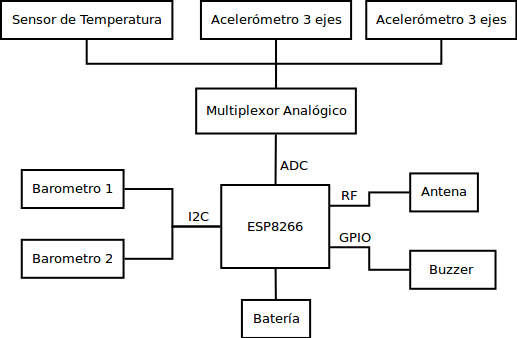
\includegraphics[width=9cm]{Imagenes/BloquesControlVuelo.png}
  \caption{Diagrama Bloques del Controlador de Vuelo}
  \label{fig:BloquesControlador}
\end{figure}

\section{Chasis del Cohete}
El objetivo inicial es desarrollar un chasis capaz de llevar como carga util un cansat hasta una altura de 1000 m. Para esto se están evaliando varios diseños para estudiar el comportamiento de los mismos. El material utilizado para el cohetete será aluminio, en su aleación mas estandar pero para evaluar los direntes diseños, se están comoenzando a desarrollar modelos de cartón.
El estudio de cada modelo de chasis se está realizando por medio de simulaciones en el software OpenRocket v15.03, en la figura \ref{fig:OpenRocket} puede verse una captura de este software con uno de los modelos evaluados.

\begin{figure}[!h]
  \centering
    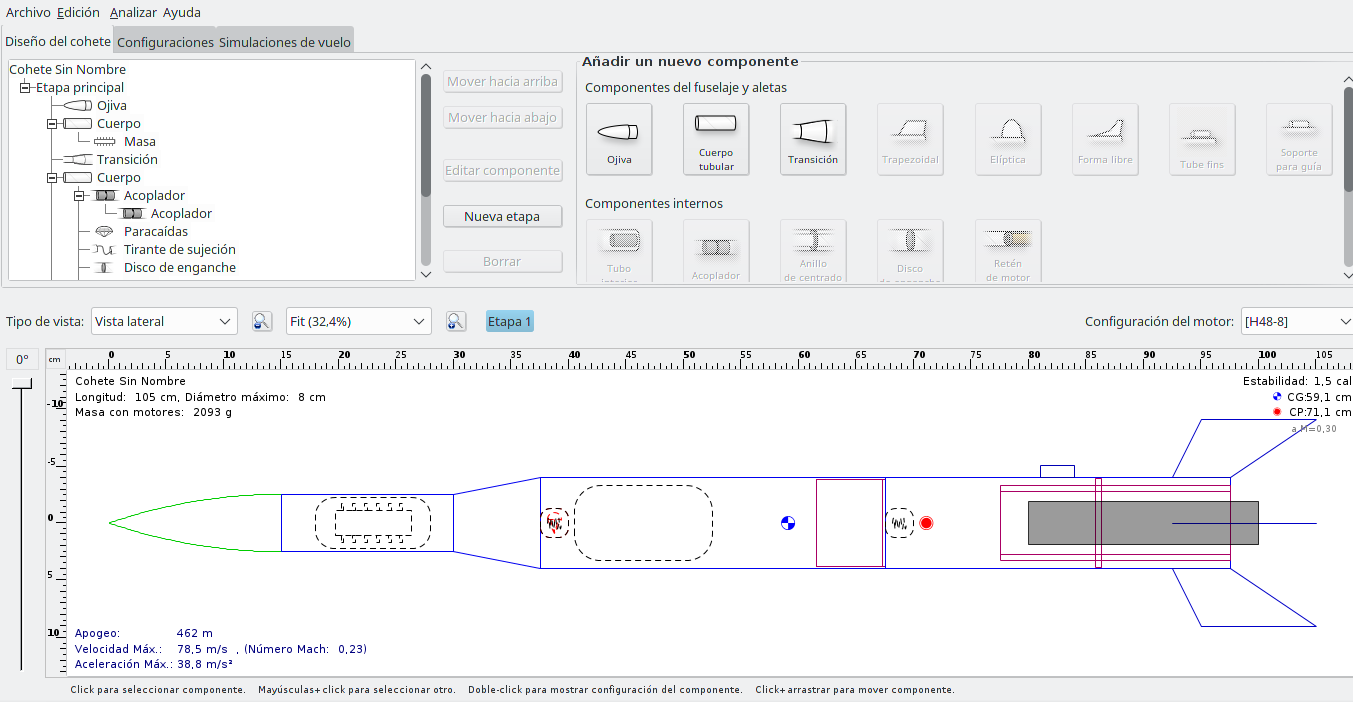
\includegraphics[width=10cm]{Imagenes/OpenRocket.png}
  \caption{Captura Open Rocket}
  \label{fig:OpenRocket}
\end{figure}

\section{Motor del Cohete}
Se decidió comenzar a desarrllor un motor de combustibe sólido, conocido como motor de azúcar. Este propelente consiste en una mezacla de azucar con sulfato de potasio y distintos aditivos para mejorar la comubstión de la mezcla. Para lograr llevar adelante un buen análisis de las distintas mezclas de propelente se está desarrollanto un pequeño banco de pruebas de motores en conjunto con el departamente de Ingenería Mecánica de la UTN.
Los primeros prototipos fueron fabricados dentro de un tubo de PVC, uno de ellos es el que se puede ver en la figura \ref{fig:Motor1} cuyo peso es de 380 g y se espera la finalización del banco de pruebas para lograr analizar su comportamiento

\begin{figure}[!h]
  \centering
    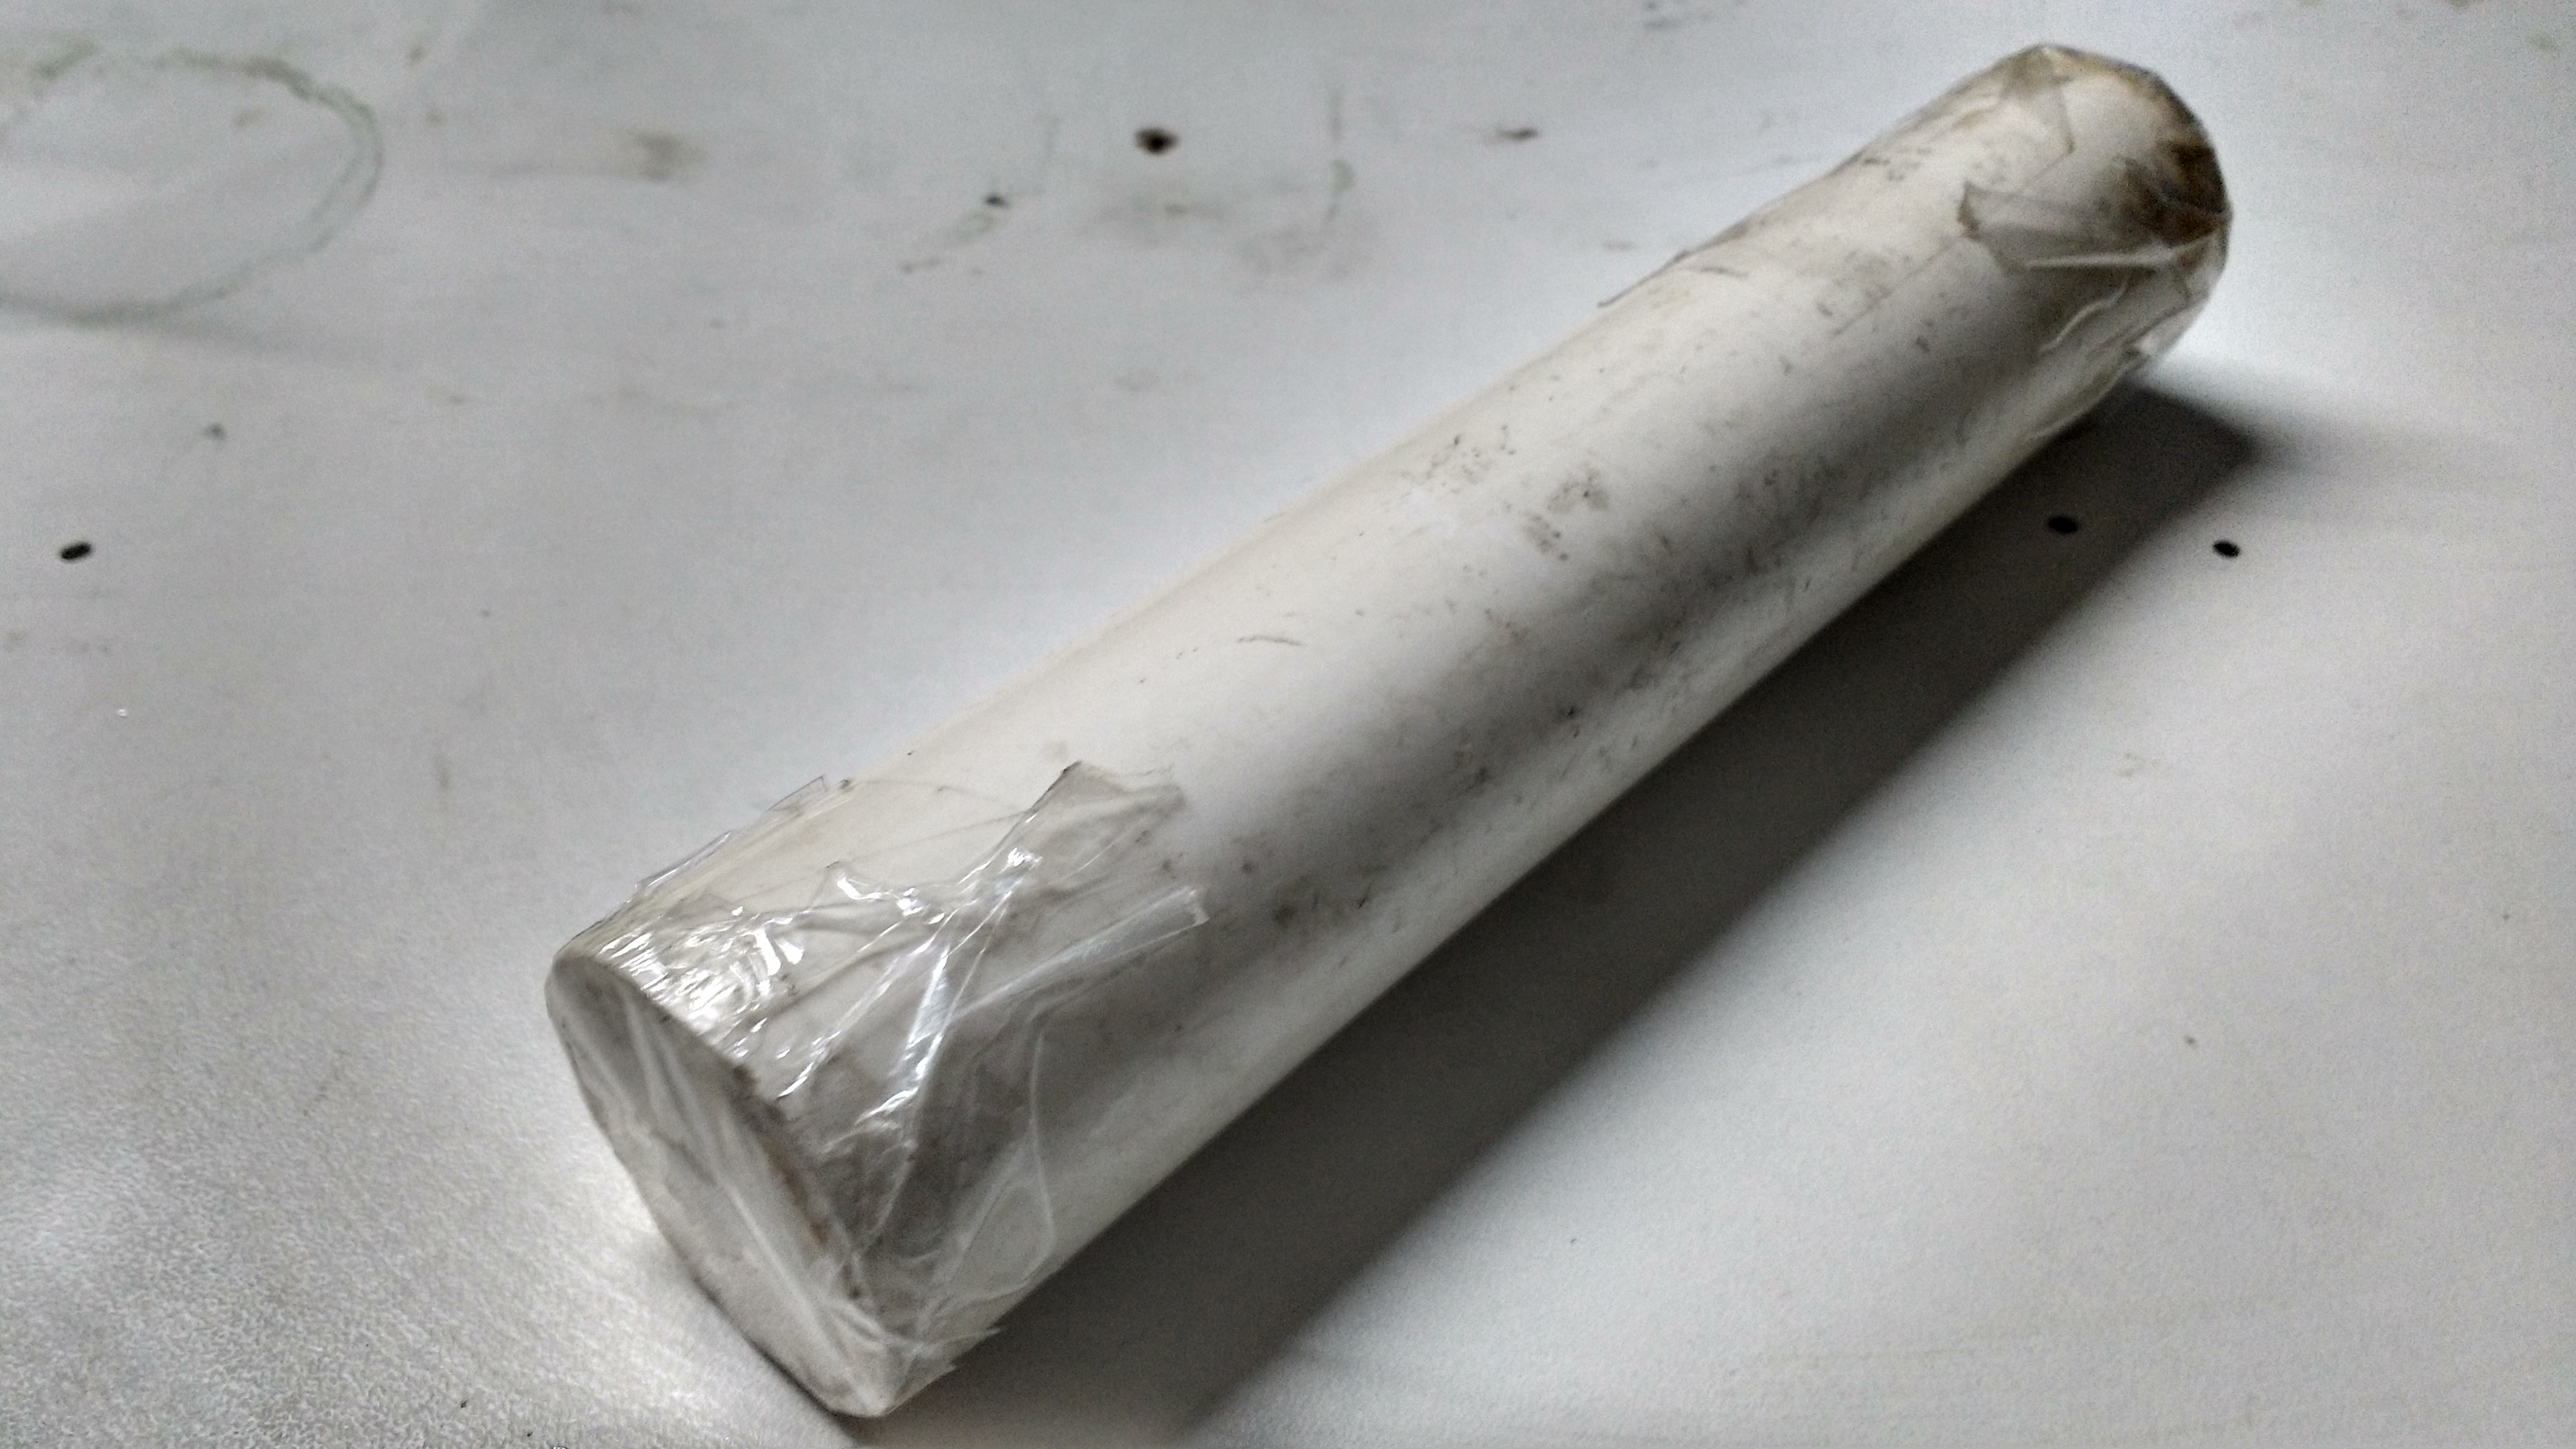
\includegraphics[width=9cm]{Imagenes/Motor.jpg}
  \caption{Primer prototipo del motor}
  \label{fig:Motor1}
\end{figure}

\subsection{Banco de Pruebas}
Consiste en un dispositivo capaz de medir la fuerza y el empuje de un motor de cohete, almacenando todos los datos en una PC. Está compuesto de una estructuira mecánica fabricada en aluminio que será colocada en una sala segura, para evitar lesiones a los operarios en caso de que ocurra algún accidente y un software cuyo objetivo es realizar la obtención y procesamiento, en tiempo real, de la información para poder tener una visión del trabajo del motor a lo largo del tiempo. Por otra parte, el mismo es capaz de exportar la información obtenida para generar una base de datos que contribuya al análisis y diseño de los motores.

\subsubsection{Estructura Mecánica}
Se está comenzando a desarrollar la estructura mecánica, la misma estará construída en aluminio y cuenta con una celda de carga para medir el empuje del motor y tres acelerómetros, para medir las vibraciones que puedan generarse tanto por el motor como por la tobera elegida. En la figura \ref{fig:Banco3d} se muestra la vista isométrica del banco que se está desarrollando.

\begin{figure}[!h]
  \centering
    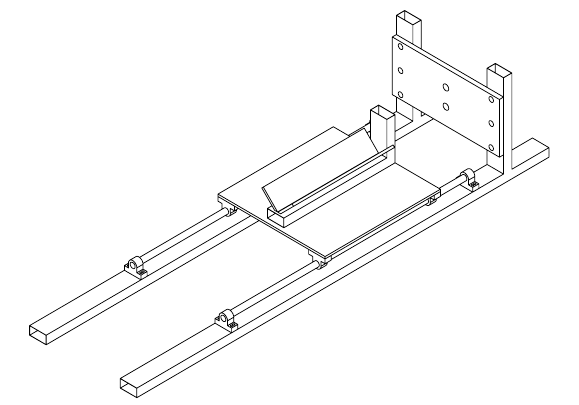
\includegraphics[width=9cm]{Imagenes/Banco3d.png}
  \caption{Prototipo Banco de pruebas}
  \label{fig:Banco3d}
\end{figure}


\subsubsection{Software de Control}
Para poder realizar este software , se decidió utilizar un lenguaje de alto nivel como Python, ya que posee numerosas herramientas y amplia disponibilidad de información. Por otro lado, posee soporte multiplataforma por lo que los programas realizados pueden ser ejecutados en múltiples sistemas operativos. La figura \ref{fig:BloquesSoftBanco}.
\begin{figure}[!h]
  \centering
    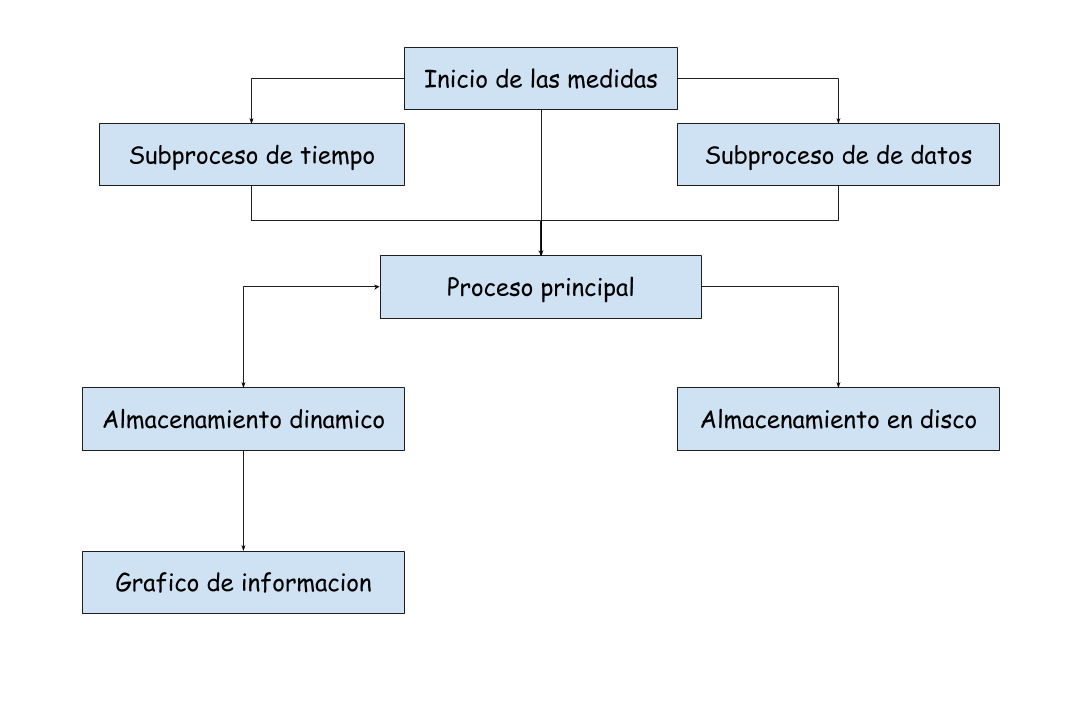
\includegraphics[width=10cm]{Imagenes/DiagramaSoftBanco.png}
  \caption{Diagrama Bloques Software}
  \label{fig:BloquesSoftBanco}
\end{figure}
Cuando se le da inicio a las mediciones, el programa inicia dos subprocesos: uno encargado de la medición del tiempo y otro encargado de la obtención de los datos. También da comienzo a el proceso principal, encargado de la coordinación entre la parte gráfica del programa y los subprocesos. El subproceso, encargado de la obtención de datos, le envía la información al proceso principal, el cual automáticamente le pide, al subproceso de tiempo, el tiempo actual desde que se inicio la medición. Luego de esto, la información se almacena en la memoria dinámica y se grafica. Al terminar la prueba del motor, los datos se almacenan en el disco con un formato conocido.
El software actualmente, como se puede ver en la figura \ref{fig:SoftBanco}, tiene un aspecto rudimentario pero, a lo largo del proyecto, se le realizarán mejoras considerables en cuanto al funcionamiento y al aspecto.
\begin{figure}[!h]
  \centering
    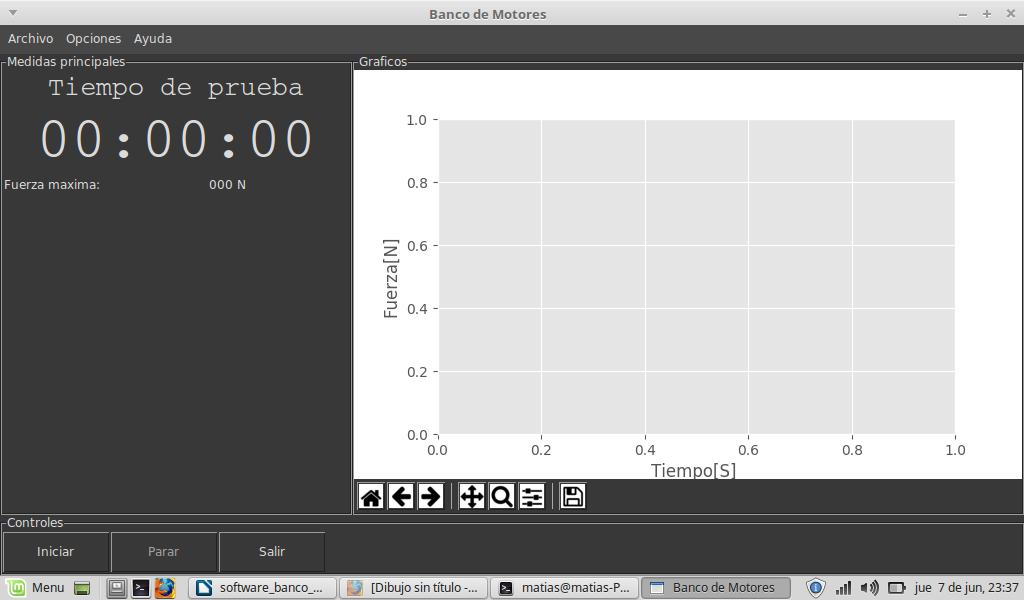
\includegraphics[width=10cm]{Imagenes/SoftBanco.png}
  \caption{Captura de Pantalla del Software}
  \label{fig:SoftBanco}
\end{figure}

\end{document}
